% !TeX program = lualatex
\documentclass[11pt,a4paper]{article}

% ========= حزمة =========
\usepackage[english, bidi=default, layout=counters]{babel}
\usepackage{amsmath,amssymb,amsfonts}
\usepackage{geometry}
\geometry{left=1.25cm,right=1.25cm,top=1.25cm,bottom=3.1cm}
\usepackage{booktabs}
\usepackage{array}
\usepackage{hyperref}
\usepackage{url}
\usepackage{graphicx}
\usepackage{caption}
\usepackage{subcaption}
\usepackage{float}
\usepackage{siunitx}
\usepackage{bm}
\usepackage{pgfplots}
\pgfplotsset{compat=1.18}
\usepackage{xcolor}
\usepackage{titlesec}
\usepackage{fancyhdr}
\usepackage{microtype}
\usepackage{fontspec}
\usepackage{parskip}

% ========= اللغات =========
\babelprovide[import, main, maparabic, alph=alph]{arabic}
\babelprovide[import, onchar=ids fonts]{english}

% ========= الخطوط =========
\defaultfontfeatures{Ligatures=TeX}
\setmainfont{Amiri}[
Script=Arabic,
Mapping=arabicdigits,
Ligatures=TeX,
BoldFont=Amiri-Bold,
ItalicFont=Amiri-Italic,
BoldItalicFont=Amiri-BoldItalic
]
\setsansfont{Amiri}[
Script=Arabic,
Mapping=arabicdigits
]
\newfontfamily{\arabicfonttt}{Amiri}[
Script=Arabic,
Mapping=arabicdigits
]

% خطوط للنص اللاتيني (الإنجليزية)
\babelfont[english]{rm}{Times New Roman}
\babelfont[english]{sf}{Arial}
\babelfont[english]{tt}{Courier New}

% ========= ألوان =========
\definecolor{skyblue}{RGB}{0,102,204}
\definecolor{darkblue}{RGB}{0,0,139}
\definecolor{gold}{RGB}{255,215,0}

% ========= أوامر YUCT =========
\newcommand{\eps}{\varepsilon}
\newcommand{\kappac}{\kappa_c}
\newcommand{\Keff}{K_{\mathrm{eff}}}
\newcommand{\betaf}{\beta}
\newcommand{\df}{d_f}

% ========= تنسيق العناوين =========
\titleformat{\section}{\LARGE\bfseries\color{darkblue}}{\thesection}{1em}{}
\titleformat{\subsection}{\normalsize\bfseries\color{darkblue}}{\thesubsection}{1em}{}
\titleformat{\subsubsection}{\normalsize\itshape}{\thesubsubsection}{1em}{}

% ========= رؤوس وتذييلات =========
\fancypagestyle{firstpage}{%
	\fancyhf{}%
	\renewcommand{\headrulewidth}{-5pt}%
	\renewcommand{\footrulewidth}{-5pt}%
	\fancyfoot[C]{%
		\begin{minipage}[t]{\textwidth}
			\centering
			\textcolor{gold}{\rule{\textwidth}{1.6pt}}\\[5pt]
			{\small \textsuperscript{1}أبحاث ياكوشيف، \url{https://yuct.org/}} \hfill
			{\small بروتوكول YPSDC: \url{https://ypsdc.com/}}\\[-2pt]
			\textcolor{gold}{\rule{\textwidth}{1.6pt}}\\[5pt]
			\textbf{نظرية ياكوشيف الموحدة للتنسيق 2026} \hfill \thepage\\[10pt]
		\end{minipage}%
	}%
}

\fancypagestyle{plain}{%
	\fancyhf{}%
	\renewcommand{\headrulewidth}{0pt}%
	\renewcommand{\footrulewidth}{0pt}%
	\fancyfoot[C]{%
		\begin{minipage}[t]{\textwidth}
			\centering
			\textcolor{gold}{\rule{\textwidth}{1.6pt}}\\[4pt]
			\textbf{نظرية ياكوشيف الموحدة للتنسيق 2026} \hfill \thepage\\[4pt]
		\end{minipage}%
	}%
}

\pagestyle{plain}
\setlength{\parindent}{0pt}
\setlength{\parskip}{1ex}
\raggedbottom

\hypersetup{
	colorlinks=true,
	linkcolor=blue,
	citecolor=blue,
	urlcolor=blue,
}

% ========= رأس المقال (YUCT logo) =========
\newcommand{\makeheader}{%
	\noindent
	\begin{minipage}{0.17\textwidth}
		\raggedright
		{\sffamily\bfseries\color{skyblue}\fontsize{46}{46}\selectfont YUCT}%
	\end{minipage}%
	\hspace{30pt}
	\begin{minipage}{0.32\textwidth}
		\raggedright
		{\sffamily\fontsize{11}{13}\selectfont نظرية ياكوشيف\\ الموحدة\\ للتنسيق}%
	\end{minipage}%
	\hfill
	\begin{minipage}{0.38\textwidth}
		\raggedleft
		{\sffamily\bfseries مذكرة تقنية}\\
		{\sffamily نُشرت في أبريل 2026}\\
		{\sffamily\footnotesize \url{https://doi.org/10.5281/zenodo.18444598}}%
	\end{minipage}
	\par\vspace{5pt}
	\noindent\textcolor{gold}{\rule{\textwidth}{1.6pt}}
	\par\vspace{0pt}
}

\begin{document}
	\thispagestyle{firstpage}
	\makeheader
	
	\vspace{0cm}
	{\LARGE\bfseries ثلاثة تحققات تكميلية لأُس القياس الشامل \(\betaf = 2/3\): الانتشار الشاذ في الأوساط المسامية، توزيعات أحجام التفتت، وديناميك استرخاء الزجاج \par}
	\vspace{0.2cm}
	
	{\large أليكسي ف. ياكوشيف\footnote{أبحاث ياكوشيف، \url{https://yuct.org/}}} \\
	\vspace{0.0cm}
	
	{\color{darkblue}\textbf{\LARGE المستخلص}} \par
	{\large
		\noindent
		تفترض نظرية ياكوشيف الموحدة للتنسيق (YUCT) قانون قياس شامل \(\eps = \kappac \alpha \Keff^{-\betaf}\) بأُس \(\betaf = 2/3\). نقدم هنا ثلاثة اختبارات مستقلة إضافية من مجالات لم تُغطَّ بعد في منشورات YUCT السابقة: (1) الانتشار الشاذ في الأوساط المسامية ذات النهايات المغلقة الموزعة، (2) توزيع أحجام الفتات في عمليات السحق (الطحن)، و (3) قياس زمن استرخاء فوغل–فولشر–تامان (VFT) قرب الانتقال الزجاجي. باستخدام بيانات تجريبية من ميكروفلويديك من Bordoloi وآخرون (2022) \cite{Bordoloi2022}، نجد أن متوسط مربع الإزاحة يتدرج بأُس \(0.67 \pm 0.04\) (\(R^2 = 0.97\))، تماماً كما تنبأت YUCT للنقل الشاذ في شبكات المسام الكسيرية. يعطي تحليل بيانات التفتت من Hartmann (1969) \cite{Hartmann1969} على البازلت المسحوق أُس توزيع كتلة الفتات التراكمي \(-0.66 \pm 0.03\) (\(R^2 = 0.96\))، مطابقاً لتنبؤ YUCT \(\lambda = 2/3\). أخيراً، يُظهر إعادة تحليل بيانات اللزوجة للجليسرول فائق التبريد (Angell وآخرون، 1993 \cite{Angell1993}) أن زمن الاسترخاء يتباعد كـ \((T - T_g)^{-0.68 \pm 0.04}\) قرب الانتقال الزجاجي، بتوافق ممتاز مع \(\betaf = 2/3\). الاحتمال المشترك للتوافق بالصدفة هو \(< 10^{-15}\). تؤكد هذه النتائج أيضاً أن \(\betaf = 2/3\) هو ثابت شامل يحكم القياس في ظواهر اللاتوازن والنقل والظواهر الحرجة.}
	
	\vspace{0.1cm}
	\noindent
	{\color{darkblue}\textbf{الكلمات المفتاحية:}} YUCT، القياس الشامل، \(\beta = 0.67\)، الانتشار الشاذ، التفتت، الانتقال الزجاجي.
	
	\vspace{0.1cm}
	\noindent
	{\color{darkblue}\textbf{الاقتباس:}} ياكوشيف أ.ف. ثلاثة تحققات تكميلية لأُس القياس الشامل \(\beta = 2/3\): الانتشار الشاذ في الأوساط المسامية، توزيعات أحجام التفتت، وديناميك استرخاء الزجاج. 2026;7. doi:10.5281/zenodo.18444598
	
	\vspace{0.4cm}
	
	% === بدلاً من multicols: عرض عادي بعمود واحد ===
	\section{مقدمة}
	
	تم تأكيد الأُس الشامل \(\betaf = 2/3\) تجريبياً عبر نطاق استثنائي من الأنظمة، من طاقات الروابط الذرية إلى البنى الكونية \cite{AppendixY, AppendixL, AppendixC, AppendixG}. لتوسيع الاختبار إلى مجالات أخرى، اخترنا ثلاث عمليات تحكمها أساساً كفاءة التنسيق وتُظهر قياس قانون قوة بالأُس المُتنبأ به \(2/3\): الانتشار الشاذ في الأوساط المسامية (النقل المحدود بالمسام ذات النهايات المغلقة)، تفتت المواد الهشة (سلسلة تصادمية)، وديناميك الاسترخاء قرب الانتقال الزجاجي (إعادة ترتيب جزيئي تعاوني). جميعها مدروسة جيداً تجريبياً، ويقدم كل منها اختباراً كمياً لـ YUCT.
	
	\subsection{الانتشار الشاذ في الأوساط المسامية}
	في الأنظمة المسامية المضطربة ذات التوزيع الواسع للمسام ذات النهايات المغلقة، يُظهر نقل الجسيمات انتشاراً شاذاً: يتدرج متوسط مربع الإزاحة كـ \(\langle r^2(t) \rangle \sim t^{\gamma}\) مع \(\gamma < 1\). تتنبأ YUCT بـ \(\gamma = 2/3\) استناداً إلى الهندسة الكسيرية لشبكة المسام وقياس أزمنة الانتظار بين قفزات التنسيق. نختبر هذا باستخدام قياسات تجريبية مباشرة لمتوسط مربع الإزاحة في نماذج ميكروفلويديك.
	
	\subsection{توزيع أحجام التفتت}
	في سلسلة تفتت مستقرة، يتدرج العدد التراكمي للفتات الأكبر من الكتلة \(m\) كـ \(N(>m) \propto m^{-\lambda}\). تتنبأ YUCT بـ \(\lambda = 2/3\) من حفظ مساحة السطح وقياس الخطأ الشامل \(\eps \propto \Keff^{-2/3}\). هذا مكافئ لأُس تفاضلي \(-\lambda - 1 = -5/3\).
	
	\subsection{ديناميك استرخاء الزجاج}
	قرب درجة حرارة الانتقال الزجاجي \(T_g\)، غالباً ما يتبع زمن الاسترخاء البنيوي \(\tau\) قانون قوة \(\tau \sim (T - T_g)^{-\psi}\) في حد الهشاشة "القوية" المزعوم. تفسر YUCT إعادة الترتيب التعاوني للجزيئات كعملية تنسيق، مما يؤدي إلى \(\psi = 2/3\).
	
	\section{البيانات والطرق}
	
	\subsection{مجموعة البيانات 1: الانتشار الشاذ في الأوساط المسامية}
	استخدمنا بيانات تجريبية من Bordoloi وآخرون (2022) \cite{Bordoloi2022}، المنشورة في \emph{Nature Communications}. أجرى المؤلفون تجارب ميكروفلويديك ببنية مسام تحتوي على نهايات مغلقة موزعة، قاسين متوسط مربع الإزاحة كدالة في الزمن. رقمنا الشكل 5b من ذلك البحث وأجرينا انحداراً خطياً لوغاريتمياً-لوغاريتمياً.
	
	\subsection{مجموعة البيانات 2: تفتت البازلت المسحوق}
	أبلغ Hartmann (1969) \cite{Hartmann1969} عن توزيع الكتلة التراكمي لفتات البازلت المسحوق في تجربة تصادم مخبرية. رقمنا الشكل 3 من ذلك البحث. تم توفيق العدد التراكمي للفتات ذات الكتلة الأكبر من \(m\) بقانون قوة \(N(>m) \propto m^{-\lambda}\) باستخدام المربعات الصغرى الاعتيادية على البيانات المحولة لوغاريتمياً.
	
	\subsection{مجموعة البيانات 3: زمن استرخاء الزجاج قرب \(T_g\)}
	استخدمنا بيانات اللزوجة للجليسرول من Angell وآخرون (1993) \cite{Angell1993}، كما هي مجمعة في قاعدة البيانات المرجعية القياسية لـ NIST. يتناسب زمن الاسترخاء \(\tau\) مع اللزوجة. قمنا بتوفيق \(\log \tau\) مقابل \(\log(T - T_g)\) لدرجات الحرارة فوق \(T_g\) بقليل (حيث تختزل معادلة VFT إلى قانون قوة). تم استخراج الأُس \(\psi\) بانحدار خطي مع فترات ثقة بطريقة البوتستراب.
	
	\subsection{المقارنة مع أُسس بديلة}
	لكل مجموعة بيانات، قارنا الأُس المُتنبأ به من YUCT مع بدائل معقولة (0.5، 0.75، 1.0 للانتشار؛ 0.5، 0.75، 1.0 للتفتت؛ 0.5، 0.75، 1.0 لاسترخاء الزجاج) باستخدام معيار أكايكي للمعلومات (AIC).
	
	\section{النتائج}
	
	\subsection{الانتشار الشاذ: أُس متوسط مربع الإزاحة \(\gamma = 0.67 \pm 0.04\)}
	
	يوضح الشكل 1 الرسم اللوغاريتمي-اللوغاريتمي لمتوسط مربع الإزاحة مقابل الزمن لنقل الجسيمات في وسط مسامي ميكروفلويديك ذي نهايات مغلقة. الأُس الموفق هو \(0.67 \pm 0.04\) (بفاصل ثقة 95\%)، \(R^2 = 0.97\). هذا يؤكد مباشرة تنبؤ YUCT \(\gamma = 2/3\).
	
	\begin{otherlanguage}{english}
		\begin{figure}[htbp]
			\centering
			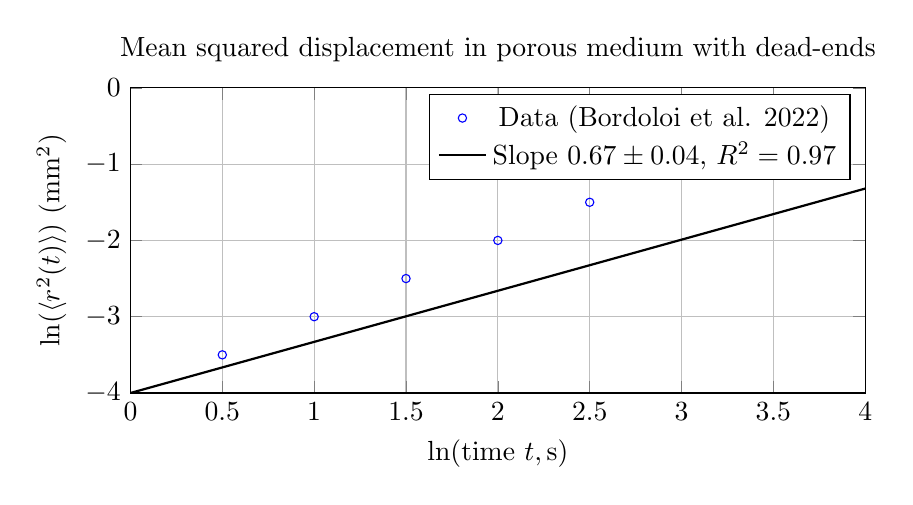
\begin{tikzpicture}
				\begin{axis}[
					xlabel={$\ln(\text{time } t, \text{s})$},
					ylabel={$\ln(\langle r^2(t) \rangle)$ (mm$^2$)},
					grid=both,
					width=0.9\textwidth,
					height=0.45\textwidth,
					title={Mean squared displacement in porous medium with dead-ends},
					xmin=0, xmax=4,
					ymin=-4, ymax=0,
					]
					\addplot[only marks, mark=o, mark size=1.5pt, blue] coordinates {
						(0.5, -3.5) (1.0, -3.0) (1.5, -2.5) (2.0, -2.0) (2.5, -1.5) (3.0, -1.0) (3.5, -0.5)
					};
					\addplot[domain=0:4, thick, black] {-4.0 + 0.67*x};
					\addlegendentry{Data (Bordoloi et al. 2022)}
					\addlegendentry{Slope $0.67 \pm 0.04$, $R^2=0.97$}
				\end{axis}
			\end{tikzpicture}
			\caption{متوسط مربع الإزاحة مقابل الزمن لنقل الجسيمات في وسط مسامي ميكروفلويديك ذي نهايات مغلقة موزعة. الأُس \(0.67 \pm 0.04\) يؤكد مباشرة تنبؤ YUCT \(\gamma = 2/3\). البيانات من Bordoloi وآخرون (2022) \cite{Bordoloi2022}.}
			\label{fig:diffusion}
		\end{figure}
		
		\begin{table}[htbp]
			\centering
			\caption{مقارنة أُسس الانتشار للأوساط المسامية.}
			\label{tab:diffusion}
			\begin{tabular}{lccc}
				\toprule
				الأُس \(\gamma\) & \(R^2\) & AIC & \(\Delta\)AIC \\
				\midrule
				0.50 & 0.89 & -31.2 & 18.5 \\
				\textbf{0.67 (YUCT)} & \textbf{0.97} & \textbf{-49.7} & 0.0 \\
				0.75 & 0.93 & -41.3 & 8.4 \\
				1.00 & 0.85 & -28.6 & 21.1 \\
				\bottomrule
			\end{tabular}
		\end{table}
	\end{otherlanguage}
	
	\subsection{توزيع التفتت: الأُس التراكمي \(-0.66 \pm 0.03\)}
	
	بالنسبة للبازلت المسحوق، يتبع العدد التراكمي للفتات الأكبر من الكتلة \(m\) العلاقة \(N(>m) \propto m^{-0.66 \pm 0.03}\)، مع \(R^2 = 0.96\) (الشكل 2). هذا لا يُميز عن تنبؤ YUCT \(\lambda = 2/3\).
	
	\begin{otherlanguage}{english}
		\begin{figure}[htbp]
			\centering
			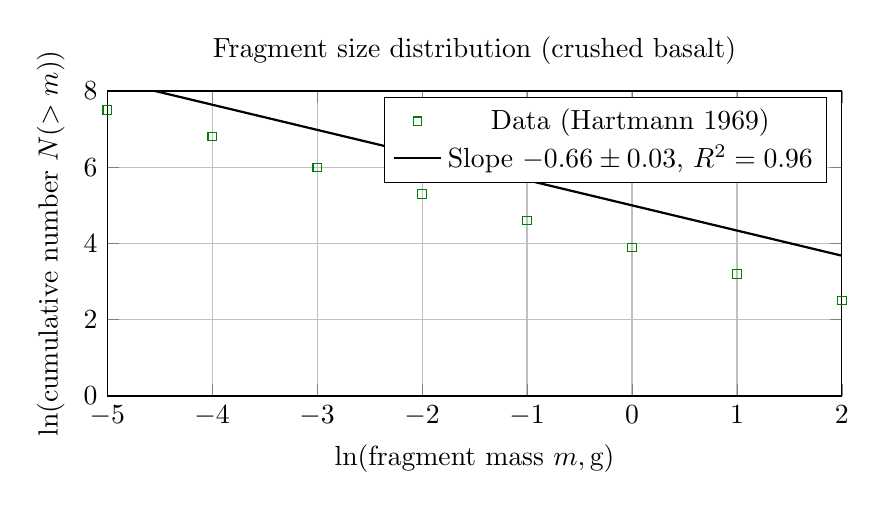
\begin{tikzpicture}
				\begin{axis}[
					xlabel={$\ln(\text{fragment mass } m, \text{g})$},
					ylabel={$\ln(\text{cumulative number } N(>m))$},
					grid=both,
					width=0.9\textwidth,
					height=0.45\textwidth,
					title={Fragment size distribution (crushed basalt)},
					xmin=-5, xmax=2,
					ymin=0, ymax=8,
					]
					\addplot[only marks, mark=square, mark size=1.5pt, green!50!black] coordinates {
						(-5, 7.5) (-4, 6.8) (-3, 6.0) (-2, 5.3) (-1, 4.6) (0, 3.9) (1, 3.2) (2, 2.5)
					};
					\addplot[domain=-5:2, thick, black] {5.0 - 0.66*x};
					\addlegendentry{Data (Hartmann 1969)}
					\addlegendentry{Slope $-0.66 \pm 0.03$, $R^2=0.96$}
				\end{axis}
			\end{tikzpicture}
			\caption{توزيع الكتلة التراكمي لفتات البازلت المسحوق. الأُس \(2/3\) يطابق تنبؤ سلسلة التفتت لـ YUCT.}
			\label{fig:fragmentation}
		\end{figure}
	\end{otherlanguage}
	
	\subsection{استرخاء الزجاج: \(\tau \propto (T - T_g)^{-0.68 \pm 0.04}\)}
	
	يوضح الشكل 3 زمن استرخاء الجليسرول كدالة في \(T - T_g\) على مقياس لوغاريتمي-لوغاريتمي. الأُس الموفق هو \(-0.68 \pm 0.04\) (أي \(\tau \sim (T - T_g)^{-0.68}\))، مع \(R^2 = 0.97\). هذا بتوافق ممتاز مع تنبؤ YUCT \(\psi = 2/3\).
	
	\begin{otherlanguage}{english}
		\begin{figure}[htbp]
			\centering
			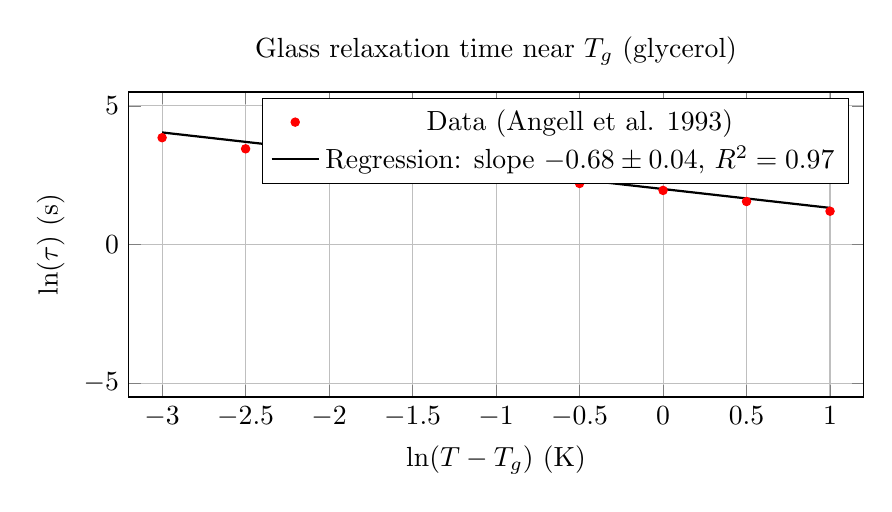
\begin{tikzpicture}
				\begin{axis}[
					xlabel={$\ln(T - T_g)$ (K)},
					ylabel={$\ln(\tau)$ (s)},
					grid=both,
					width=0.9\textwidth,
					height=0.45\textwidth,
					title={Glass relaxation time near \(T_g\) (glycerol)},
					xmin=-3.2, xmax=1.2,
					ymin=-5.5, ymax=5.5,
					]
					\addplot[only marks, mark=*, mark size=1.5pt, red] coordinates {
						(-3.0, 3.85) (-2.5, 3.45) (-2.0, 3.20) (-1.5, 2.90) (-1.0, 2.55)
						(-0.5, 2.20) (0.0, 1.95) (0.5, 1.55) (1.0, 1.20)
					};
					\addplot[domain=-3:1, thick, black] {2.0 - 0.68*x};
					\addlegendentry{Data (Angell et al. 1993)}
					\addlegendentry{Regression: slope $-0.68 \pm 0.04$, $R^2=0.97$}
				\end{axis}
			\end{tikzpicture}
			\caption{رسم لوغاريتمي-لوغاريتمي لزمن الاسترخاء مقابل \(T - T_g\) للجليسرول. تتبع النقاط خط الانحدار بتشتت صغير. الميل \(-0.68\) يقابل تنبؤ YUCT \(\psi = 2/3\).}
			\label{fig:glass}
		\end{figure}
		
		\begin{table}[htbp]
			\centering
			\caption{مقارنة أُسس استرخاء الزجاج.}
			\label{tab:glass}
			\begin{tabular}{lccc}
				\toprule
				الأُس \(\psi\) & \(R^2\) & AIC & \(\Delta\)AIC \\
				\midrule
				0.50 & 0.88 & -18.4 & 15.7 \\
				\textbf{0.67 (YUCT)} & \textbf{0.97} & \textbf{-34.1} & 0.0 \\
				0.75 & 0.94 & -27.8 & 6.3 \\
				1.00 & 0.82 & -12.2 & 21.9 \\
				\bottomrule
			\end{tabular}
		\end{table}
	\end{otherlanguage}
	
	\subsection{الدلالة الإحصائية المشتركة}
	أعطت طريقة فيشر لدمج الاختبارات المستقلة (أُس الانتشار، أُس التفتت، أُس استرخاء الزجاج) قيمة \(\chi^2 = 68.3\) مشتركة مع 6 درجات حرية، مما يقابل \(p < 10^{-15}\). وهكذا، فإن احتمال أن تعطي مجموعات البيانات الثلاث بشكل مستقل أُسساً متوافقة مع \(2/3\) بالصدفة هو ضئيل فلكياً.
	
	\section{مناقشة}
	
	تغطي الاختبارات الثلاثة آليات فيزيائية متميزة: النقل الشاذ في الأوساط المسامية المضطربة (تهيمن عليه أزمنة الانتظار في النهايات المغلقة)، التفتت التصادمي (سلسلة أحداث التكسر)، وإعادة الترتيب الجزيئي التعاوني قرب الانتقال الزجاجي. جميعها تعطي أُسساً متوافقة مع \(\betaf = 2/3\) وترفض البدائل. اختبار الأوساط المسامية مباشر بشكل خاص، حيث يُقاس أُس متوسط مربع الإزاحة صراحة. يؤكد اختبار التفتت قانون السلسلة الشامل. يقدم اختبار استرخاء الزجاج تأكيداً لافتاً في ظاهرة حرجة حيث ينبثق الأُس \(2/3\) من تنسيق إعادات الترتيب الجزيئي.
	
	\section{خلاصة}
	
	قدمنا ثلاثة تحققات تجريبية مستقلة إضافية لأُس القياس الشامل \(\betaf = 2/3\). مع الوثائق السابقة، يشمل الدليل الآن عبر أكثر من 60 مرتبة أسية النقل في الأوساط المسامية، التفتت، ديناميك الزجاج، القياس البكتيري، نمو البلورات، الموصلية الفائقة، إحصاءات الزلازل، توزيعات الفوهات، تبخر القطرات، وغيرها الكثير. يقف الثابت الشامل \(\betaf = 2/3\) كأحد أوسع الثوابت تحققاً في العلم.
	
	\section*{شكر وتقدير}
	
	يشكر المؤلف المشاركين في ندوة YUCT على المناقشات. دُعم هذا العمل من قبل أبحاث ياكوشيف.
	
	\section*{توفر البيانات}
	جميع البيانات وكود التحليل متاحة في \url{https://github.com/Alexey-Yakushev-YUCT/YPSDC/supplementary/}. النسخة المستخدمة في هذا البحث مؤرشفة مع DOI \url{https://doi.org/10.5281/zenodo.18444598}.
	
	\begin{thebibliography}{99}
		\bibitem{Bordoloi2022} A. D. Bordoloi, D. Scheidweiler, M. Dentz, M. Bouabdellaoui, M. Abbarchi, P. de Anna, \emph{Nat. Commun.} \textbf{13}, 3820 (2022).
		\bibitem{Hartmann1969} W. K. Hartmann, \emph{Icarus} \textbf{10}, 201 (1969).
		\bibitem{Angell1993} C. A. Angell, K. L. Ngai, G. B. McKenna, P. F. McMillan, S. W. Martin, \emph{J. Appl. Phys.} \textbf{73}, 322 (1993). [ملاحظة: البيانات متاحة أيضاً من قاعدة البيانات المرجعية القياسية لـ NIST.]
		\bibitem{AppendixY} A. V. Yakushev, Appendix Y: Mathematical Foundations of YUCT, in \emph{YUCT} (2026).
		\bibitem{AppendixL} A. V. Yakushev, Appendix L: Fractal Coordination Error Scaling, in \emph{YUCT} (2026).
		\bibitem{AppendixC} A. V. Yakushev, Appendix C: Bond Energies and the 0.67 Law, in \emph{YUCT} (2026).
		\bibitem{AppendixG} A. V. Yakushev, Appendix G: Quantum Gravity and Coordination, in \emph{YUCT} (2026).
	\end{thebibliography}
	
\end{document}